\documentclass[tikz]{standalone}

\usetikzlibrary{calc,positioning}

\tikzset{agent/.style={%
        circle,
        minimum size=2mm,inner xsep=1.2mm,inner ysep=1.2mm,
        anchor=center,
        very thick,
        draw}}

\tikzset{link/.style={very thick,>=stealth,rounded corners}}


\begin{document}

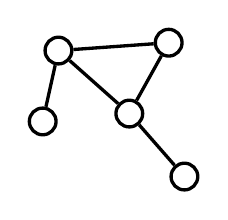
\begin{tikzpicture}
  \node [agent] (1) at (0,0) {};
  \node [agent] (2) at (1.4,0.1) {};
  \node [agent] (3) at (-0.2,-.9) {};
  \node [agent] (4) at (0.9,-.8) {};
  \node [agent] (5) at (1.6,-1.6) {};  % \node [agent] (5) at (2,-.6) {};
  \draw [link] (1) -- (2);
  \draw [link] (1) -- (4);
  \draw [link] (1) -- (3);
  \draw [link] (2) -- (4);
  \draw [link] (4) -- (5);
\end{tikzpicture}

\end{document}